\documentclass[11pt,a4paper]{book}

% ===================================
% Essential Packages
% ===================================
\usepackage[utf8]{inputenc}
\usepackage[T1]{fontenc}
\usepackage[top=2.5cm, bottom=1.5cm, left=1.5cm, right=1.5cm]{geometry}
\usepackage{amsmath, amssymb, amsfonts}
\allowdisplaybreaks
\usepackage{graphicx}
\usepackage{color}
\usepackage{xcolor}
\usepackage{hyperref}
\usepackage{enumitem}
\usepackage[most]{tcolorbox}  % loads enhanced, breakable, skins, etc.
\usepackage{fancyhdr}
\usepackage{booktabs}
\usepackage{array}
\usepackage{longtable}
\usepackage{multirow}
\usepackage{tikz}
\usepackage{mdframed}
\usepackage{listings}
\usepackage{colortbl}
\usepackage{subcaption}  % for sub-figures
\usepackage{float}
\usepackage{gensymb}
\usepackage{calligra}      % Calligraphy font
\usepackage[export]{adjustbox}
\usepackage[font=small, labelfont=bf]{caption}
\captionsetup[longtable]{width=\textwidth, justification=centering}
\usepackage{titlesec}

% TikZ libraries for advanced graphics
\usetikzlibrary{shapes, arrows, positioning, decorations.pathmorphing, decorations.markings, calc}
\usetikzlibrary{patterns, shadows, backgrounds}

% Color definitions - Soft, elegant palette
\definecolor{primaryblue}{HTML}{6BA3C8}         % Accent blue
\definecolor{secondaryblue}{HTML}{A8D8E8}       % Lighter sky blue
\definecolor{lightgray}{HTML}{F5F5F0}           % Cream white
\definecolor{darkgray}{HTML}{3D3D3D}            % Charcoal
\definecolor{successgreen}{HTML}{A8D8E8}        % Sky blue (replacing green)
\definecolor{warningorange}{HTML}{E8B4B8}       % Soft rose pink
\definecolor{dangerred}{HTML}{E8B4B8}           % Soft rose pink
\definecolor{navyblue}{HTML}{4A3C3A}            % Deep brown
\definecolor{primaryteal}{HTML}{6BA3C8}         % Accent blue
\definecolor{digitalgreen}{HTML}{A8D8E8}        % Sky blue
\definecolor{techpurple}{HTML}{B8A8C8}          % Muted violet
\definecolor{cyanorange}{HTML}{E8B4B8}          % Soft rose pink
\definecolor{custompurple}{HTML}{B8A8C8}        % Muted violet
\definecolor{chaptercolor}{HTML}{2F6FA3}        % Deeper accent blue
\definecolor{sectioncolor}{HTML}{5C524F}        % Dark warm gray/brown
\definecolor{subsectioncolor}{HTML}{C46A75}     % Rich rose pink
\definecolor{subsubsectioncolor}{HTML}{7C68A6}  % Deeper muted violet

% New tcolorbox colors - Soft, distinct palette
\definecolor{mintgreen}{HTML}{A8D5BA}           % Soft mint green for definitionbox
\definecolor{softpeach}{HTML}{F4C2A3}           % Soft peach for formulabox
\definecolor{sagegreen}{HTML}{B8C9B3}           % Soft sage green for infobox
\definecolor{softlavender}{HTML}{D4C5E8}        % Soft lavender for questionanswerbox
\definecolor{softcoral}{HTML}{F5A5A8}           % Soft coral for derivationbox

% --- Prevent automatic uppercase in headers ---
\renewcommand{\chaptermark}[1]{%
  \markboth{Chapter \thechapter: #1}{}}
\renewcommand{\sectionmark}[1]{%
  \markright{Section \thesection: #1}}

% --- Header and footer ---
\usepackage{fancyhdr}
\pagestyle{fancy}
\fancyhf{} % clear all fields

% --- Normal pages header ---
\fancyhead[L]{%
    \begin{minipage}[t]{0.48\textwidth}
    \raggedright
    \adjustbox{max width=\linewidth}{\textcolor{darkgray}{\textbf{\leftmark}}}%
    \end{minipage}}
\fancyhead[R]{%
    \begin{minipage}[t]{0.48\textwidth}
    \raggedleft
    \adjustbox{max width=\linewidth}{\textcolor{darkgray}{\textbf{\rightmark}}}%
    \end{minipage}}

% Centered footer page number and signature
\fancyfoot[C]{\textcolor{darkgray}{\thepage}}
\fancyfoot[R]{\tiny\textcalligra{\textcolor{dangerred}{Miad}}}

% Header line
\renewcommand{\headrulewidth}{2pt}
\renewcommand{\headrule}{\hbox to\headwidth{\color{primaryblue}\leaders\hrule height \headrulewidth\hfill}}

% Chapter starting pages style
\fancypagestyle{plain}{%
    \fancyhf{} % clear headers/footers
    \fancyfoot[C]{\textcolor{darkgray}{\thepage}} % centered page number
    \fancyfoot[R]{\tiny\textcalligra{\textcolor{dangerred}{Miad}}} % keep signature
    \renewcommand{\headrulewidth}{0pt} % no header line
}

\setcounter{secnumdepth}{4}  % 0=chapter, 1=section, 2=subsection, 3=subsubsection

% Chapter style - Clean and prominent
\titleformat{\chapter}
  {\normalfont\Huge\bfseries\color{chaptercolor}}
  {Chapter \thechapter.}
  {1em}
  {}
  [\vspace{2pt}\textcolor{chaptercolor}{\titlerule[2.5pt]}]

% Section style - Clean numbered format
\titleformat{\section}
  {\normalfont\huge\bfseries\color{sectioncolor}}
  {\thesection}
  {1em}
  {}

% Subsection style - Simple and clear
\titleformat{\subsection}
  {\normalfont\LARGE\bfseries\color{subsectioncolor}}
  {\thesubsection}
  {1em}
  {}

% Subsubsection style - Minimal decoration
\titleformat{\subsubsection}
  {\normalfont\Large\bfseries\color{subsubsectioncolor}}
  {\thesubsubsection}
  {1em}
  {}

% Spacing adjustments
\titlespacing*{\chapter}{0pt}{0pt}{2.3ex plus .2ex}
\titlespacing*{\section}{0pt}{3.5ex plus 1ex minus .2ex}{2.3ex plus .2ex}
\titlespacing*{\subsection}{0pt}{3.25ex plus 1ex minus .2ex}{1.5ex plus .2ex}
\titlespacing*{\subsubsection}{0pt}{3.25ex plus 1ex minus .2ex}{1.5ex plus .2ex}

% ===============================
% Custom tcolorbox Environments
% ===============================

% Note Box (Soft Mint Green)
\newenvironment{definitionbox}[1][Definition]{
    \begin{tcolorbox}[
        enhanced,
        breakable,
        colback=primaryblue!10,
        colframe=primaryblue!150,
        title=#1,
        fonttitle=\bfseries,
        sharp corners,
        boxrule=0.8pt,
        left=8pt,
        right=8pt,
        top=6pt,
        bottom=6pt
    ]
}{
    \end{tcolorbox}
}

% Formula Box (Soft Peach)
\newenvironment{formulabox}[1][Formula]{
    \begin{tcolorbox}[
        enhanced,
        breakable,
        colback=softcoral!10,
        colframe=softcoral!200,
        title=#1,
        fonttitle=\bfseries,
        coltitle=white,
        sharp corners,
        boxrule=1pt,
        left=8pt,
        right=8pt,
        top=6pt,
        bottom=6pt
    ]
}{
    \end{tcolorbox}
}

% Success Box (Soft Sage Green)
\newenvironment{infobox}[1][For more understanding]{
    \begin{tcolorbox}[
        enhanced,
        breakable,
        colback=mintgreen!10,
        colframe=mintgreen!200,
        title=#1,
        fonttitle=\bfseries,
        sharp corners,
        boxrule=0.8pt,
        left=8pt,
        right=8pt,
        top=6pt,
        bottom=6pt
    ]
}{
    \end{tcolorbox}
}

% Define QnA counter that resets every chapter
\newcounter{qna}[chapter]
\renewcommand{\theqna}{\thechapter.\arabic{qna}}

% Question Answer Box (Soft Lavender)
\newenvironment{questionanswerbox}{
    \refstepcounter{qna}% step counter and make it referenceable
    \begin{tcolorbox}[
        enhanced,
        breakable,
        colback=softlavender!10,
        colframe=softlavender!200,
        title={Example~\theqna}, % automatic numbering
        fonttitle=\bfseries,
        coltitle=white,
        colbacktitle=softlavender!200,
        sharp corners,
        boxrule=1pt,
        left=8pt,
        right=8pt,
        top=6pt,
        bottom=6pt
    ]
}{
    \end{tcolorbox}
}

% Definition Box (Soft Coral)
\newenvironment{derivationbox}[1][Derivation]{
    \begin{tcolorbox}[
        enhanced,
        breakable,
        colback=softpeach!10,
        colframe=softpeach!200,
        title=#1,
        fonttitle=\bfseries,
        sharp corners,
        boxrule=0.8pt,
        left=10pt,
        right=10pt,
        top=8pt,
        bottom=8pt
    ]
}{
    \end{tcolorbox}
}



% % Custom bullet points
% \setlist[itemize,1]{label=\textcolor{primaryblue}{$\bullet$}, leftmargin=*}
% \setlist[itemize,2]{label=\textcolor{darkgray}{$\circ$}, leftmargin=*}
% \setlist[itemize,3]{label=\textcolor{primaryblue}{$\rightarrow$}, leftmargin=*}

% % Numbered lists
% \setlist[enumerate,1]{label=\textcolor{primaryblue}{\arabic*.}, leftmargin=*}
% \setlist[enumerate,2]{label=\textcolor{darkgray}{(\alph*)}, leftmargin=*}

% Hyperlink settings
\hypersetup{
    colorlinks=true,
    linkcolor=primaryblue,
    urlcolor=primaryblue,
    citecolor=primaryblue
}

% Title page information
\title{\textcolor{primaryblue}{\Huge\textbf{Course Notes Template}}}
\author{\textcolor{darkgray}{\Large Your Name}}
\date{\textcolor{darkgray}{\Large\today}}

\begin{document}
\newpage
\setcounter{page}{1}

% Table of Contents
\tableofcontents
\newpage

% Main Content Starts Here
\chapter{Introduction to Information Theory}
\section{Basics}
\begin{definitionbox}[Data]
    Statistical value without meaning.
\end{definitionbox}

\begin{definitionbox}[Information]
    Information is any entity or form that resolves uncertainty or provides the answer to a question of some kind.
\end{definitionbox}

\noindent $\rightarrow$ Information theory deals with -
\begin{itemize}
    \item The measure of some information.
    \item The information capacity of channel.
    \item Coding.
\end{itemize}

\noindent $\rightarrow$ Two fundamental things of communication theory - 
\begin{itemize}
    \item Entropy (H)
    \item Channel capacity (C)
\end{itemize}

\section{Information and Probability Relation}
\begin{formulabox}
    \[I \propto \frac{1}{p}\]

    where - 
    \begin{itemize}
        \item I = Information
        \item p = Probability
    \end{itemize}
\end{formulabox}

\begin{infobox}
    \begin{itemize}
        \item If probability is 100\% then Information I = 0
        \item If any data contains uncertainty then that's information
        \item Uncertainty is showed by Probability
    \end{itemize}
\end{infobox}

\begin{definitionbox}[Self-information]
\begin{itemize}
    \item Consider a discrete random variable \( X \) with the possible outcomes \( X_i \), where \( i = 1, 2, 3, \dots, L \).
    \item The self-information of the event \( X = X_i \) is defined as:
            \[
            I(X_i) = \log \left( \frac{1}{p(X_i)} \right) = - \log p(X_i)
            \]
    or
    \[
    I(X_i) = - \log_2 p(X_i)
    \]
    Here Base = 2 because the data is in binary.
\end{itemize}
\end{definitionbox}

\begin{infobox}[Information and Probability]
    \begin{itemize}
        \item A high probability event converges with less information. Means p $\uparrow$ $\rightarrow$ I $\downarrow$
        \item For an event \( p(X_i) = 1 \), the self-information \( I(X_i) = 0 \).
        \item A lower probability implies a higher degree of uncertainty, and vice versa. Means p $\uparrow$ $\rightarrow$ uncertainty $\downarrow$ or p $\downarrow$ $\rightarrow$ uncertainty $\uparrow$
    \end{itemize}
\end{infobox}

\begin{questionanswerbox}
    If the probability of an event \( p(X_i) = 0.5 \), the self-information is:
    \[
    I(X_i) = - \log_2 0.5 = 1 \text{ bit}.
    \]
    Here the unit of information is bit.
\end{questionanswerbox}

\section{Units of Information}
\begin{itemize}
    \item Base $\rightarrow$ 2 then unit $\rightarrow$ bit (binary digits)
    \item Base $\rightarrow$ e then unit $\rightarrow$ nats
    \item Base $\rightarrow$ 10 then unit $\rightarrow$ decimal digits
\end{itemize}

\section{Information and Probability Relation (Extended)}

$\rightarrow$ \textbf{Fundamental Relationship} 
\begin{itemize}
    \item For independent events, information is additive while probabilities are multiplicative.
    \item This motivates the logarithmic relationship.
\end{itemize}  

\begin{derivationbox}[Cause of Logarithm for Information]
\begin{itemize}[label=$\rightarrow$]
    \item Consider three independent events with probabilities \(p_1, p_2, p_3\).
    \item \textbf{For probabilities (multiplicative):}
    \[
    p_{\text{total}} = p_1 \cdot p_2 \cdot p_3
    \]
    \item \textbf{For information (additive):}
    \[
    I_{\text{total}} = I_1 + I_2 + I_3
    \]
    \item  Since-
    \begin{align*}
    I &= \log \frac{1}{p_{X_i}} = \log \frac{1}{p_{total}}\\
    I &= \log \frac{1}{p_1 \cdot p_2 \cdot p_3} \\
    &= \log \frac{1}{p_1} + \log \frac{1}{p_2} + \log \frac{1}{p_3}
    \end{align*}
    \item If all probabilities are same then-
    \begin{align*}
        I &= \sum_{n} \log \frac{1}{p_n}\\
        I &= -\sum_{n} \log p_n
    \end{align*}
\end{itemize}
\textbf{Key insight:} When probability is same for all events, information is averaged equally across all possibilities.
\end{derivationbox}

\section{Application of Information}
\begin{itemize}
    \item Source coding $\rightarrow$ Data compression
    \item Channel coding $\rightarrow$ To make correction if noise gets added in the channel
    \item To know the limitation of bandwidth its necessary to know information theory
\end{itemize}

\section{Importance of Information Theory}
\begin{enumerate}
    \item To determine the amount of informant can be transmitted through band limited noisy channel
    \item How much error can be reduced and corrected
    \item Source coding is done to compress data
    \item Channel coding is done to recover data by adding extra bits
    \item Amount of compression depends on the amount of information
\end{enumerate}

\begin{questionanswerbox}
    \textbf{Q:} Why is log compression chosen for measuring information?\\
    \textbf{A:}\\
    Logarithmic compression is preferred for measuring information because it has key properties that match our understanding of uncertainty and information:

    \begin{itemize}
        \item \textbf{Additivity of Information:} 
            \begin{itemize}
                \item The total information from independent events is the sum of the individual information values.
                \item For two independent events with probabilities \( P_1 \) and \( P_2 \), the total information is:
                \[
                I = \log_2 \left( P_1 \cdot P_2 \right) = \log_2 P_1 + \log_2 P_2
                \]
            \end{itemize}
        
        \item \textbf{Compression of High Probability Events:} 
            \begin{itemize}
                \item Events with higher probabilities contain less information, while events with lower probabilities contain more.
                \item The information for an event \( X_i \) with probability \( P(X_i) \) is given by:
                \[
                I(X_i) = -\log_2 P(X_i)
                \]
                \item Example: For \( P_1 = P_2 = \frac{1}{6} \), the combined information for two independent events is:
                \[
                I = \log_2 \left( \frac{1}{6} \cdot \frac{1}{6} \right) = -2 \log_2 6
                \]
            \end{itemize}
        
        \item \textbf{Scalability with Uncertainty:} 
            \begin{itemize}
                \item Logarithmic functions scale so that larger differences in probability lead to larger differences in information.
                \item Example: If \( P(X_i) = \frac{1}{2} \), the self-information is:
                \[
                I(X_i) = -\log_2 \left( \frac{1}{2} \right) = 1 \text{ bit}
                \]
            \end{itemize}

        \item \textbf{Intuitive Interpretation:} 
            \begin{itemize}
                \item High probability events have low self-information (less surprise), and low probability events have high self-information (more surprise).
                \item For two independent events \( X_1 \) and \( X_2 \) with probabilities \( P_1 \) and \( P_2 \), the total information is:
                \[
                I_{\text{total}} = I_1 + I_2 = -\log_2 P_1 - \log_2 P_2
                \]
            \end{itemize}

    \end{itemize}

    \textbf{Conclusion:} The logarithmic function is chosen because it naturally describes how we perceive and measure uncertainty, making it an ideal tool for quantifying information in probabilistic systems.
\end{questionanswerbox}

\chapter{Entropy Relative-Entropy and Mutual-Information}

\begin{formulabox}[Probability and Information Formula]
    \begin{align*}
        p_{\text{total}} &= p_1 \cdot p_2 \cdot p_3\\
        I_{\text{total}} &= I_1 + I_2 + I_3\\
    \end{align*}
    If all of the probability is the same then-
    \begin{align*}
        I &= -\sum_{n}\log p_n
    \end{align*}
\end{formulabox}

\begin{questionanswerbox}
    \textbf{Example: 2-bit Binary System}
    \begin{itemize}[label=$\rightarrow$]
        \item Consider a 2-bit system with 4 possible outcomes: 00, 01, 10, 11
        \item  Each outcome has probability:
    \[
    p_{00}, p_{01}, p_{10}, p_{11}
    \]
    \item  The total information is:
    \begin{align*}
    I &= I_1 + I_2 + I_3 + I_4 \\
    &= \log \frac{1}{p_1} + \log \frac{1}{p_2} + \log \frac{1}{p_3} + \log \frac{1}{p_4} \\
    &= \log \frac{1}{p_{00}} + \log \frac{1}{p_{01}} + \log \frac{1}{p_{10}} + \log \frac{1}{p_{11}} \\
    &= (-\log p_{00}) + (-\log p_{01}) + (-\log p_{10}) + (-\log p_{11})\\
    I &= -\sum_{n}\log p_n
    \end{align*}
    \item Therefore, entropy (average information) is:
    \[
    H = -\sum_{n} p_n \log p_n
    \]
    \end{itemize}
    \textbf{Conclusion:} When probability is the same for all events, information is distributed evenly across all outcomes (maximum entropy). This average is called entropy.
\end{questionanswerbox}

\begin{formulabox}[Entropy Formula]
\begin{align*}
    H &= -\sum_{n} p_n \log p_n\\
    I &= -\sum_{n}\log p_n
\end{align*}
\end{formulabox}

\begin{infobox}[Probability Information and Entropy Understanding]
    \begin{itemize}
        \item $p \propto \frac{1}{I}$ and $p \propto \frac{1}{H}$
        \item $H \propto I$
        \item p $\uparrow$ $\rightarrow$ I $\downarrow$ $\rightarrow$ H $\downarrow$
        \item p, I, H are never -ve
    \end{itemize}
\end{infobox}

\begin{formulabox}[Extreme Cases]
    \begin{enumerate}
        \item When \(P = 1\) (certain event):
        \[
        I = \log \frac{1}{1} = 0 \quad \text{(no information)}
        \]
        
        \item When \(P = 0\) (impossible event):
        \[
        I = \log \frac{1}{0} = \infty \quad \text{(infinite information/surprise)}
        \]
        
        \item For maximum entropy with \(L\) outcomes:
        \[
        P = \frac{1}{L} \text{ for all outcomes} \quad \Rightarrow \quad H_{\max} = \log L
        \]
    \end{enumerate}
\end{formulabox}

\section{Entropy}

\begin{definitionbox}[Entropy]
    \begin{itemize}
        \item Entropy is a measure of uncertainty or randomness of a random variable.
        \item For a discrete random variable \(X\) with alphabet \(\mathcal{X}\) and probability mass function \(p(x) = \Pr(X = x)\), the entropy \(H(X)\) is defined as:
    \[
    H(X) = -\sum_{x \in \mathcal{X}} p(x) \log_2 p(x)
    \]
    \item Where-
    \begin{itemize}
        \item p(x) = Expectation = Probability
    \end{itemize}
    \end{itemize}
\end{definitionbox}

\subsection{Key Points about Entropy}
\begin{itemize}
        \item Entropy represents the \textbf{average information} content
        \item Higher entropy means higher uncertainty
        \item Unit is \textbf{bit} when logarithm base is 2, \textbf{nat} when base is \(e\)
        \item Entropy depends only on the probability distribution, not on actual values
        \item Convention: \(0 \log 0 = 0\) (justified by continuity as \(x \log x \to 0\) when \(x \to 0\))
    \end{itemize}

\begin{formulabox}[Alternative Form of Entropy]
    The entropy can also be interpreted as the expected value of self-information:
    \[
    H(X) = E_p\left[\log \frac{1}{p(X)}\right] = E_p[I(X)]
    \]
    where \(I(x) = \log \frac{1}{p(x)} = -\log p(x)\) is the self-information of outcome \(x\).
\end{formulabox}

\subsection{Properties of Entropy}
\begin{formulabox}[Property 1: Non-negativity]
    \[
    H(X) \geq 0
    \]
    \textbf{Proof:} Since \(0 \leq p(x) \leq 1\), we have \(\log p(x) \leq 0\), thus \(-p(x) \log p(x) \geq 0\) for all \(x\).
\end{formulabox}

\begin{formulabox}[Property 2: Base Conversion]
    \[
    H_b(X) = (\log_b a) \cdot H_a(X)
    \]
    The base of the logarithm in entropy can be changed by multiplying by the appropriate conversion factor.
    
    \textbf{Proof:} \(\log_b p = \log_b a \cdot \log_a p\)
\end{formulabox}

\begin{formulabox}[Property 3: Maximum Uncertainty/Entropy]
    For a random variable \(X\) with \(L\) possible outcomes, entropy is maximized when all outcomes are equally likely:
    \[
    H(X) \leq \log_2 L
    \]
    Equality holds when \(p(x_i) = \frac{1}{L}\) for all \(i = 1, 2, \ldots, L\).
\end{formulabox}

\begin{infobox}[Understanding Maximum Entropy]
    \begin{itemize}
        \item When \(P = \frac{1}{2}\), uncertainty is maximum
        \item The graph of \(H(p)\) versus \(p\) is a concave curve with maximum at \(p = 0.5\)
        \item This makes intuitive sense: a fair coin has maximum uncertainty
    \end{itemize}
\end{infobox}

\begin{questionanswerbox}
    \textbf{Q: Binary Random Variable Entropy when p = $\frac{1}{2}$}
    \[\text{Let} X = \begin{cases} 1 & \text{with probability } p \\ 0 & \text{with probability } 1-p \end{cases}\]  Find H(X).
\\
 \textbf{A:}\\
 We know - 
 \begin{align*}
     H(X) &= -\sum_{x \in \mathcal{X}} p(x) \log_2 p(x)\\
    &= -p \log_2 p - (1-p) \log_2(1-p)\\
    &= -\frac{1}{2} \log_2 \frac{1}{2} - (1-\frac{1}{2}) \log_2(1-\frac{1}{2})\\
    &= -\frac{1}{2} \log_2 \frac{1}{2} - (\frac{1}{2}) \log_2(\frac{1}{2})\\
    &= -\log_2 \frac{1}{2} = \log_2 2 = 1
 \end{align*}
    
    In particular, \(H(X) = 1\) bit when \(p = 1/2\).
    \begin{figure}[H]
        \centering
        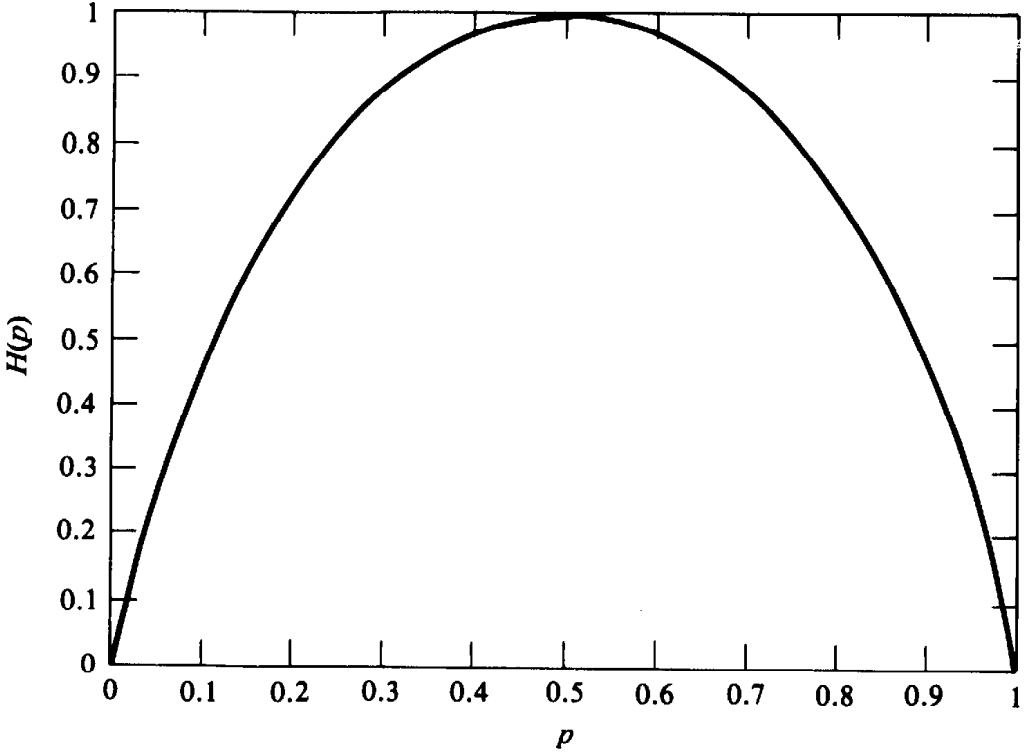
\includegraphics[width=0.5\linewidth]{Figures/H(p) versus p..png}
        \caption{H(p) versus p.}
        \label{fig:H(p) versus p.}
    \end{figure}
    
    The function \(H(p)\) is concave and symmetric around \(p = 0.5\), reaching its maximum of 1 bit at this point. When \(p = 0\) or \(p = 1\), there is no uncertainty, so \(H = 0\).
\end{questionanswerbox}

\begin{questionanswerbox}
    \textbf{Example 2: Four-Symbol Source}
    
    Let \(X = \begin{cases}
    a & \text{with probability } 1/2 \\
    b & \text{with probability } 1/4 \\
    c & \text{with probability } 1/8 \\
    d & \text{with probability } 1/8
    \end{cases}\)
    
    The entropy is:
    \begin{align*}
    H(X) &= -\sum_{x \in \mathcal{X}} p(x) \log_2 p(x)\\
    &= -\frac{1}{2}\log \frac{1}{2} - \frac{1}{4}\log \frac{1}{4} - \frac{1}{8}\log \frac{1}{8} - \frac{1}{8}\log \frac{1}{8} \\
    &= -\frac{1}{2}(-1) - \frac{1}{4}(-2) - \frac{1}{8}(-3) - \frac{1}{8}(-3) \\
    &= \frac{1}{2} + \frac{1}{2} + \frac{3}{8} + \frac{3}{8} \\
    &= \frac{7}{4} = 1.75 \text{ bits}
    \end{align*}
    
    \textbf{Note:} If all probabilities were equal (\(p = 1/4\) for all), then:
    \[
    H(X) = -4 \cdot \frac{1}{4}\log_2 \frac{1}{4} = \log_2 4 = 2 \text{ bits}
    \]
    
    This shows that when probabilities are not uniform, entropy is less than maximum, and information is maximized with equal probabilities.
\end{questionanswerbox}

\subsection{Joint Entropy}

\begin{definitionbox}[Joint Entropy]
    The joint entropy \(H(X,Y)\) of a pair of discrete random variables \((X,Y)\) with joint distribution \(p(x,y)\) is defined as:
    \[
    H(X,Y) = -\sum_{x \in \mathcal{X}} \sum_{y \in \mathcal{Y}} p(x,y) \log p(x,y)
    \]
    
    Alternatively:
    \[
    H(X,Y) = -E \log p(X,Y)
    \]
\end{definitionbox}

\begin{infobox}[Properties of Joint Entropy]
    \begin{itemize}
        \item \(H(X,Y) \geq 0\)
        \item \(H(X,Y) = H(X) + H(Y)\) if and only if \(X\) and \(Y\) are independent
        \item \(H(X,Y) \leq H(X) + H(Y)\) (equality for independence)
    \end{itemize}
\end{infobox}

\subsection{Conditional Entropy}

\begin{definitionbox}[Conditional Entropy]
    The conditional entropy \(H(Y|X)\) measures the average uncertainty remaining in \(Y\) when \(X\) is known:
    \[
    H(Y|X) = \sum_{x \in \mathcal{X}} p(x) \sum_{y \in \mathcal{Y}} p(y|x) \log p(y|x)
    \]
    
    Equivalently:
    \[
    H(Y|X) = -E \log p(Y|X)
    \]
\end{definitionbox}

\subsection{Chain Rule for Entropy}
\begin{formulabox}[Chain Rule for Entropy]
    \[
    H(X,Y) = H(X) + H(Y|X)
    \]
    
    \textbf{Interpretation:} Joint Entropy = Marginal Entropy + Conditional Entropy
\end{formulabox}

\begin{derivationbox}[Proof of Chain Rule]
    Starting from the definition of joint entropy:
    \begin{align*}
    H(X,Y) &= -\sum_{x \in \mathcal{X}} \sum_{y \in \mathcal{Y}} p(x,y) \log p(x,y) \\
    &= -\sum_{x,y} p(x,y) \log [p(x)p(y|x)] \\
    &= -\sum_{x,y} p(x,y) \log p(x) - \sum_{x,y} p(x,y) \log p(y|x) \\
    &= -\sum_{x} p(x) \log p(x) - \sum_{x,y} p(x,y) \log p(y|x) \\
    &= H(X) + H(Y|X)
    \end{align*}
\end{derivationbox}

\begin{questionanswerbox}
    \textbf{Example: Joint Distribution - Complete Calculation}
    
    Let \((X,Y)\) have the following joint distribution:
    
    \begin{center}
    \begin{tabular}{c|cccc|c}
    \(Y \backslash X\) & 1 & 2 & 3 & 4 & \(p(Y)\)\\ \hline
    1 & 1/8 & 1/16 & 1/32 & 1/32 & 1/4\\
    2 & 1/16 & 1/8 & 1/32 & 1/32 & 1/4\\
    3 & 1/16 & 1/16 & 1/16 & 1/16 & 1/4\\
    4 & 1/4 & 0 & 0 & 0 & 1/4\\ \hline
    \(p(X)\) & 1/2 & 1/4 & 1/8 & 1/8 & 1
    \end{tabular}
    \end{center}
    
    \textbf{Step 1: Calculate Marginal Entropy \(H(X)\)}
    
    Marginal distribution of \(X\): \(p(X) = \left(\frac{1}{2}, \frac{1}{4}, \frac{1}{8}, \frac{1}{8}\right)\)
    
    \begin{align*}
    H(X) &= -\sum_{x} p(x) \log_2 p(x) \\
    &= -\frac{1}{2}\log_2 \frac{1}{2} - \frac{1}{4}\log_2 \frac{1}{4} - \frac{1}{8}\log_2 \frac{1}{8} - \frac{1}{8}\log_2 \frac{1}{8} \\
    &= -\frac{1}{2}(-1) - \frac{1}{4}(-2) - \frac{1}{8}(-3) - \frac{1}{8}(-3) \\
    &= \frac{1}{2} + \frac{2}{4} + \frac{3}{8} + \frac{3}{8} \\
    &= \frac{4}{8} + \frac{4}{8} + \frac{3}{8} + \frac{3}{8} = \frac{14}{8} = \frac{7}{4} \text{ bits}
    \end{align*}
    
    \textbf{Step 2: Calculate Marginal Entropy \(H(Y)\)}
    
    Marginal distribution of \(Y\): \(p(Y) = \left(\frac{1}{4}, \frac{1}{4}, \frac{1}{4}, \frac{1}{4}\right)\)
    
    \begin{align*}
    H(Y) &= -\sum_{y} p(y) \log_2 p(y) \\
    &= -4 \times \frac{1}{4}\log_2 \frac{1}{4} \\
    &= -4 \times \frac{1}{4} \times (-2) \\
    &= 2 \text{ bits}
    \end{align*}
    
    \textbf{Step 3: Calculate Conditional Entropy \(H(X|Y)\) and Joint Entropy \(H(X,Y)\)}
    
    The conditional entropy formula is:
    \[
    H(X|Y) = \sum_{i=1}^{4} p(Y=i) \cdot H(X|Y=i)
    \]
    
    This means: "Average the entropy of X for each fixed value of Y, weighted by probability of that Y."

    \begin{formulabox}[Bayes' rule]
        To find \(H(X|Y=i)\), we need the conditional probabilities \(p(X=j|Y=i)\).
    
    Using Bayes' rule: \(p(X=j|Y=i) = \frac{p(X=j, Y=i)}{p(Y=i)}\)
    \end{formulabox}
    
    \hrulefill
    
    \textbf{When \(Y=1\):} \(p(Y=1) = \frac{1}{4}\)
    
    Conditional probabilities from the joint table:
    \begin{align*}
    p(X=1|Y=1) &= \frac{p(X=1,Y=1)}{p(Y=1)} = \frac{1/8}{1/4} = \frac{1}{2} \\
    p(X=2|Y=1) &= \frac{p(X=2,Y=1)}{p(Y=1)} = \frac{1/16}{1/4} = \frac{1}{4} \\
    p(X=3|Y=1) &= \frac{p(X=3,Y=1)}{p(Y=1)} = \frac{1/32}{1/4} = \frac{1}{8} \\
    p(X=4|Y=1) &= \frac{p(X=4,Y=1)}{p(Y=1)} = \frac{1/32}{1/4} = \frac{1}{8}
    \end{align*}
    
    \textbf{Verification:} \(\frac{1}{2} + \frac{1}{4} + \frac{1}{8} + \frac{1}{8} = 1\) ✓
    
    Now calculate entropy:
    \begin{align*}
    H(X|Y=1) &= -\sum_{j=1}^{4} p(X=j|Y=1) \log_2 p(X=j|Y=1) \\
    &= -\frac{1}{2}\log_2\frac{1}{2} - \frac{1}{4}\log_2\frac{1}{4} - \frac{1}{8}\log_2\frac{1}{8} - \frac{1}{8}\log_2\frac{1}{8} \\
    &= -\frac{1}{2}(-1) - \frac{1}{4}(-2) - \frac{1}{8}(-3) - \frac{1}{8}(-3) \\
    &= \frac{1}{2} + \frac{1}{2} + \frac{3}{8} + \frac{3}{8} = \frac{7}{4} \text{ bits}
    \end{align*}
    
    \hrulefill
    
    \textbf{When \(Y=2\):} \(p(Y=2) = \frac{1}{4}\)
    
    Conditional probabilities:
    \begin{align*}
    p(X=1|Y=2) &= \frac{1/16}{1/4} = \frac{1}{4}, \quad
    p(X=2|Y=2) = \frac{1/8}{1/4} = \frac{1}{2} \\
    p(X=3|Y=2) &= \frac{1/32}{1/4} = \frac{1}{8}, \quad
    p(X=4|Y=2) = \frac{1/32}{1/4} = \frac{1}{8}
    \end{align*}
    
    Entropy:
    \begin{align*}
    H(X|Y=2) &= -\frac{1}{4}\log_2\frac{1}{4} - \frac{1}{2}\log_2\frac{1}{2} - \frac{1}{8}\log_2\frac{1}{8} - \frac{1}{8}\log_2\frac{1}{8} \\
    &= \frac{1}{2} + \frac{1}{2} + \frac{3}{8} + \frac{3}{8} = \frac{7}{4} \text{ bits}
    \end{align*}
    
    \hrulefill
    
    \textbf{When \(Y=3\):} \(p(Y=3) = \frac{1}{4}\)
    
    Conditional probabilities:
    \begin{align*}
    p(X=1|Y=3) &= \frac{1/16}{1/4} = \frac{1}{4}, \quad
    p(X=2|Y=3) = \frac{1/16}{1/4} = \frac{1}{4} \\
    p(X=3|Y=3) &= \frac{1/16}{1/4} = \frac{1}{4}, \quad
    p(X=4|Y=3) = \frac{1/16}{1/4} = \frac{1}{4}
    \end{align*}
    
    Entropy (uniform distribution):
    \begin{align*}
    H(X|Y=3) &= -4 \times \frac{1}{4}\log_2\frac{1}{4} = -4 \times \frac{1}{4} \times (-2) = 2 \text{ bits}
    \end{align*}
    
    \hrulefill
    
    \textbf{When \(Y=4\):} \(p(Y=4) = \frac{1}{4}\)
    
    Conditional probabilities:
    \begin{align*}
    p(X=1|Y=4) &= \frac{1/4}{1/4} = 1, \quad
    p(X=2|Y=4) = \frac{0}{1/4} = 0 \\
    p(X=3|Y=4) &= \frac{0}{1/4} = 0, \quad
    p(X=4|Y=4) = \frac{0}{1/4} = 0
    \end{align*}
    
    Entropy (deterministic - no uncertainty):
    \begin{align*}
    H(X|Y=4) &= -1 \cdot \log_2 1 - 0 \cdot \log_2 0 - 0 \cdot \log_2 0 - 0 \cdot \log_2 0 \\
    &= 0 \text{ bits (X is always 1 when Y=4)}
    \end{align*}
    
    \hrulefill
    
    \textbf{Now combine all cases:}
    \begin{align*}
    H(X|Y) &= \sum_{i=1}^{4} p(Y=i) \cdot H(X|Y=i) \\
    &= p(Y=1) \cdot H(X|Y=1) + p(Y=2) \cdot H(X|Y=2) \\
    &\quad + p(Y=3) \cdot H(X|Y=3) + p(Y=4) \cdot H(X|Y=4) \\
    &= \frac{1}{4} \times \frac{7}{4} + \frac{1}{4} \times \frac{7}{4} + \frac{1}{4} \times 2 + \frac{1}{4} \times 0 \\
    &= \frac{7}{16} + \frac{7}{16} + \frac{8}{16} + 0 \\
    &= \frac{22}{16} = \frac{11}{8} \text{ bits}
    \end{align*}
    
    \textbf{Finally, using the chain rule:}
    \[
    H(X,Y) = H(Y) + H(X|Y) = 2 + \frac{11}{8} = \frac{16}{8} + \frac{11}{8} = \frac{27}{8} \text{ bits}
    \]
    
    \textbf{Step 4: Calculate \(H(Y|X)\)}
    
    Similarly, using: \(H(X,Y) = H(X) + H(Y|X)\)
    \[
    H(Y|X) = H(X,Y) - H(X) = \frac{27}{8} - \frac{7}{4} = \frac{27}{8} - \frac{14}{8} = \frac{13}{8} \text{ bits}
    \]
    
    \textbf{Summary of Results:}
    \begin{itemize}
        \item \(H(X) = \frac{7}{4} = 1.75\) bits
        \item \(H(Y) = 2\) bits
        \item \(H(X,Y) = \frac{27}{8} = 3.375\) bits
        \item \(H(X|Y) = \frac{11}{8} = 1.375\) bits
        \item \(H(Y|X) = \frac{13}{8} = 1.625\) bits
    \end{itemize}
    
    \textbf{Verification:}
    \begin{itemize}
        \item \(H(X,Y) = H(X) + H(Y|X) = \frac{7}{4} + \frac{13}{8} = \frac{14}{8} + \frac{13}{8} = \frac{27}{8}\) ✓
        \item \(H(X,Y) = H(Y) + H(X|Y) = 2 + \frac{11}{8} = \frac{16}{8} + \frac{11}{8} = \frac{27}{8}\) ✓
    \end{itemize}
\end{questionanswerbox}

\begin{infobox}[Important Observations]
    \begin{itemize}
        \item \(H(Y|X) \neq H(X|Y)\) — Conditional entropies are generally not equal
        \item However, \(H(X) - H(X|Y) = H(Y) - H(Y|X)\) — This symmetric property is mutual information \(I(X;Y)\), explored in the next section
        \item \(H(X|Y) < H(X)\) — Knowing \(Y\) reduces uncertainty about \(X\)
        \item \(H(Y|X) < H(Y)\) — Knowing \(X\) reduces uncertainty about \(Y\)
    \end{itemize}
\end{infobox}

\section{Relative Entropy}
    \begin{itemize}
        \item Entropy \(H(X)\) measures the uncertainty of a single random variable
        \item Relative entropy extends this concept to measure the "distance" between two probability distributions
    \end{itemize}

\begin{definitionbox}[Relative Entropy(Kullback-Leibler Divergence)]
    The \textbf{relative entropy} or \textbf{Kullback-Leibler (KL) divergence} between two probability mass functions \(p(x)\) and \(q(x)\) is defined as:
    \[
    D(p \| q) = \sum_{x \in \mathcal{X}} p(x) \log \frac{p(x)}{q(x)}
    \]
    
    Equivalently, in expectation form:
    \[
    D(p \| q) = E_p \log \frac{p(X)}{q(X)}
    \]
    
    \textbf{Convention:} Based on continuity arguments:
    \begin{itemize}
        \item \(0 \log \frac{0}{q} = 0\)
        \item \(p \log \frac{p}{0} = \infty\)
    \end{itemize}
\end{definitionbox}

\begin{infobox}[Interpretation of Relative Entropy (Coding Perspective)]
    \begin{itemize}
        \item The relative entropy \(D(p \| q)\) is a measure of the inefficiency of assuming that the distribution is \(q\) when the true distribution is \(p\)
        \item If we knew the true distribution \(p\), we could construct a code with average description length \(H(p)\)
        \item If instead we used a code designed for distribution \(q\), we would need \(H(p) + D(p \| q)\) bits on average to describe the random variable
        \item Thus, \(D(p \| q)\) represents the \textbf{extra bits} needed due to using the wrong distribution
    \end{itemize}
\end{infobox}

\subsection{Properties of Relative Entropy}
    \begin{enumerate}
        \item \textbf{Non-negativity:} \(D(p \| q) \geq 0\)
        \item \textbf{Zero condition:} \(D(p \| q) = 0\) if and only if \(p(x) = q(x)\) for all \(x\)
        \item \textbf{Asymmetry:} \(D(p \| q) \neq D(q \| p)\) in general
        \item \textbf{Not a metric:} Does not satisfy the triangle inequality and is not symmetric
    \end{enumerate}
    
\begin{questionanswerbox}
    \textbf{Example 2.3.1: Binary Distributions with Different Parameters}
    
    Let \(\mathcal{X} = \{0, 1\}\) and consider two distributions \(p\) and \(q\) on \(\mathcal{X}\).
    
    \textbf{Given:}
    \begin{itemize}
        \item Distribution \(p\): \(p(0) = 1-r\), \(p(1) = r\)
        \item Distribution \(q\): \(q(0) = 1-s\), \(q(1) = s\)
    \end{itemize}

    \begin{formulabox}[General Formulas]
    
    The relative entropy from \(p\) to \(q\):
    \[
    D(p \| q) = (1-r) \log \frac{1-r}{1-s} + r \log \frac{r}{s}
    \]
    
    The relative entropy from \(q\) to \(p\):
    \[
    D(q \| p) = (1-s) \log \frac{1-s}{1-r} + s \log \frac{s}{r}
    \]
    \end{formulabox}
    
    \hrulefill
    
    \textbf{Special Case 1: Equal Distributions}
    
    If \(r = s\), then both distributions are identical:
    \[
    D(p \| q) = D(q \| p) = 0
    \]
    \textbf{Observation:} This confirms that relative entropy is zero when the distributions match.
    
    \hrulefill
    
    \textbf{Special Case 2: Specific Values}
    
    Let \(r = 1/2\) and \(s = 1/4\). Then:
    
    \textbf{Calculate \(D(p \| q)\):}
    \begin{align*}
    D(p \| q) &= (1-r) \log \frac{1-r}{1-s} + r \log \frac{r}{s} \\
    &= \frac{1}{2} \log \frac{1/2}{3/4} + \frac{1}{2} \log \frac{1/2}{1/4} \\
    &= \frac{1}{2} \log \frac{2}{3} + \frac{1}{2} \log 2 \\
    &= \frac{1}{2} \left(\log 2 - \log 3\right) + \frac{1}{2} \log 2 \\
    &= \frac{1}{2} \log 2 - \frac{1}{2} \log 3 + \frac{1}{2} \log 2 \\
    &= \log 2 - \frac{1}{2} \log 3 \\
    &= 1 - \frac{1}{2} \log 3 \\
    &\approx 1 - 0.7925 = 0.2075 \text{ bits}
    \end{align*}
    
    \textbf{Calculate \(D(q \| p)\):}
    \begin{align*}
    D(q \| p) &= (1-s) \log \frac{1-s}{1-r} + s \log \frac{s}{r} \\
    &= \frac{3}{4} \log \frac{3/4}{1/2} + \frac{1}{4} \log \frac{1/4}{1/2} \\
    &= \frac{3}{4} \log \frac{3}{2} + \frac{1}{4} \log \frac{1}{2} \\
    &= \frac{3}{4} (\log 3 - \log 2) + \frac{1}{4} (- \log 2) \\
    &= \frac{3}{4} \log 3 - \frac{3}{4} \log 2 - \frac{1}{4} \log 2 \\
    &= \frac{3}{4} \log 3 - \log 2 \\
    &= \frac{3}{4} \log 3 - 1 \\
    &\approx 1.1887 - 1 = 0.1887 \text{ bits}
    \end{align*}
    
    \textbf{Observation:}
    \[
    D(p \| q) = 0.2075 \text{ bits} \neq D(q \| p) = 0.1887 \text{ bits}
    \]
    
    This demonstrates that \textbf{KL divergence is asymmetric} — the "distance" from \(p\) to \(q\) is different from the "distance" from \(q\) to \(p\).
\end{questionanswerbox}

\section{Mutual Information}
\begin{itemize}
    \item Mutual information quantifies the amount of information one random variable contains about another
    \item These concepts are fundamental for understanding information flow and coding efficiency
\end{itemize}

\begin{definitionbox}[Mutual Information]
    Consider two random variables \(X\) and \(Y\) with joint probability mass function \(p(x,y)\) and marginal probability mass functions \(p(x)\) and \(p(y)\). 
    
    The \textbf{mutual information} \(I(X;Y)\) is the relative entropy between the joint distribution and the product distribution \(p(x)p(y)\):
    \[
    I(X;Y) = \sum_{x \in \mathcal{X}} \sum_{y \in \mathcal{Y}} p(x,y) \log \frac{p(x,y)}{p(x)p(y)}
    \]
    
    Equivalently:
    \[
    I(X;Y) = D(p(x,y) \| p(x)p(y))
    \]
    
    Or in expectation form:
    \[
    I(X;Y) = E_{p(x,y)} \log \frac{p(X,Y)}{p(X)p(Y)}
    \]
\end{definitionbox}

\begin{infobox}[Interpretation of Mutual Information]
    \begin{itemize}
        \item Mutual information measures the amount of information one random variable contains about another
        \item It quantifies the \textbf{reduction in uncertainty} of one variable due to knowledge of the other
        \item \(I(X;Y)\) represents how much knowing \(Y\) reduces uncertainty about \(X\) (and vice versa)
        \item It measures the dependence between \(X\) and \(Y\)
        \item When \(X\) and \(Y\) are independent: \(I(X;Y) = 0\)
    \end{itemize}
\end{infobox}

\subsection{Relationship with Entropy}

\begin{formulabox}[Theorem 2.4.1: Mutual Information and Entropy]
    The mutual information can be expressed in several equivalent forms:
    
    \begin{align}
    I(X;Y) &= H(X) - H(X|Y) \tag{2.43}\\
    I(X;Y) &= H(Y) - H(Y|X) \tag{2.44}\\
    I(X;Y) &= H(X) + H(Y) - H(X,Y) \tag{2.45}\\
    I(X;Y) &= I(Y;X) \quad \text{(symmetric)} \tag{2.46}\\
    I(X;X) &= H(X) \tag{2.47}
    \end{align}
    
    \textbf{Interpretations:}
    \begin{itemize}
        \item \textbf{Equation (2.43):} Mutual information = Uncertainty in \(X\) − Uncertainty in \(X\) given \(Y\)
        \item \textbf{Equation (2.44):} Mutual information = Uncertainty in \(Y\) − Uncertainty in \(Y\) given \(X\)
        \item \textbf{Equation (2.45):} Mutual information = Sum of marginal entropies − Joint entropy
        \item \textbf{Equation (2.46):} Mutual information is symmetric
        \item \textbf{Equation (2.47):} A variable contains all information about itself
    \end{itemize}
\end{formulabox}

\subsubsection{Venn Diagram Representation (Visual Understanding)}

    The relationship between \(H(X)\), \(H(Y)\), \(H(X,Y)\), \(H(X|Y)\), \(H(Y|X)\), and \(I(X;Y)\) can be visualized as a Venn diagram (Figure 2.2):
    
    \begin{figure}[H]
        \centering
        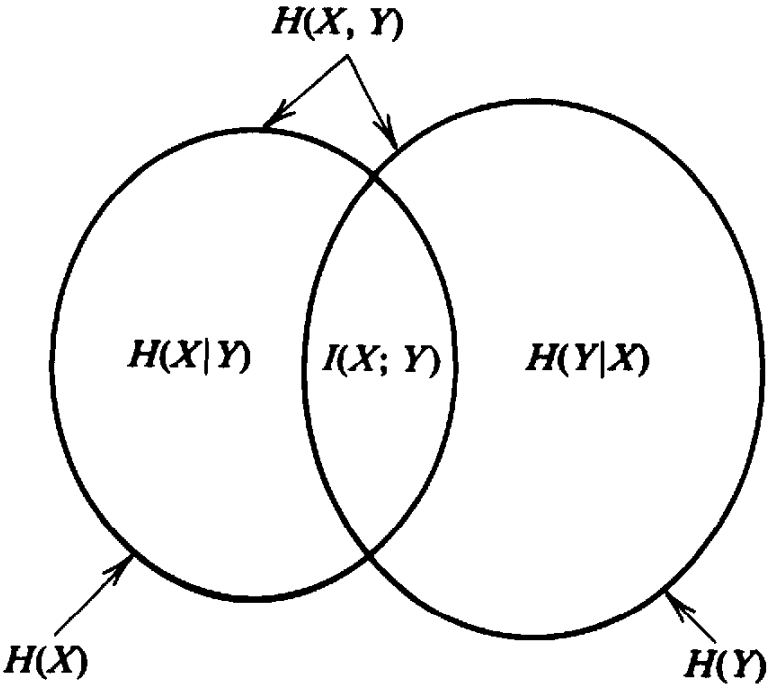
\includegraphics[width=0.3\linewidth]{Figures/Relationship between entropy and mutual information.png}
        \caption{Relationship between entropy and mutual information.}
        \label{fig:Relationship between entropy and mutual information.}
    \end{figure}
    
    \textbf{Key Observations:}
    \begin{itemize}
        \item \textbf{Left circle}: Total uncertainty in \(X\) is \(H(X)\)
        \item \textbf{Right circle}: Total uncertainty in \(Y\) is \(H(Y)\)
        \item \textbf{Intersection}: Shared information is \(I(X;Y)\)
        \item \textbf{Left only}: Uncertainty in \(X\) after knowing \(Y\) is \(H(X|Y)\)
        \item \textbf{Right only}: Uncertainty in \(Y\) after knowing \(X\) is \(H(Y|X)\)
        \item \textbf{Total area}: Joint uncertainty is \(H(X,Y) = H(X|Y) + I(X;Y) + H(Y|X)\)
    \end{itemize}
    
    The mutual information corresponds to the intersection — the information that \(X\) and \(Y\) share.

\subsection{Properties of Mutual Information}
    \begin{enumerate}
        \item \textbf{Non-negativity:} \(I(X;Y) \geq 0\) 
        \begin{itemize}
            \item Equality holds when \(X\) and \(Y\) are independent
        \end{itemize}
        
        \item \textbf{Symmetry:} \(I(X;Y) = I(Y;X)\)
        
        \item \textbf{Independence condition:} \(I(X;Y) = 0\) if and only if \(X\) and \(Y\) are independent
        
        \item \textbf{Upper bound:} \(I(X;Y) \leq \min\{H(X), H(Y)\}\)
        \begin{itemize}
            \item Mutual information cannot exceed the entropy of either variable
        \end{itemize}
        
        \item \textbf{Self-information:} \(I(X;X) = H(X)\)
        \begin{itemize}
            \item A variable contains complete information about itself
        \end{itemize}
    \end{enumerate}

\subsection{Example: Calculating Mutual Information}

\begin{questionanswerbox}
    \textbf{Example: Mutual Information from Joint Distribution}
    
    Using the joint distribution from Chapter 2:
    
    \begin{center}
    \begin{tabular}{c|cccc|c}
    \(Y \backslash X\) & 1 & 2 & 3 & 4 & \(p(Y)\)\\ \hline
    1 & 1/8 & 1/16 & 1/32 & 1/32 & 1/4\\
    2 & 1/16 & 1/8 & 1/32 & 1/32 & 1/4\\
    3 & 1/16 & 1/16 & 1/16 & 1/16 & 1/4\\
    4 & 1/4 & 0 & 0 & 0 & 1/4\\ \hline
    \(p(X)\) & 1/2 & 1/4 & 1/8 & 1/8 & 1
    \end{tabular}
    \end{center}
    
    \textbf{Previously calculated values:}
    \begin{itemize}
        \item \(H(X) = \frac{7}{4} = 1.75\) bits
        \item \(H(Y) = 2\) bits
        \item \(H(X,Y) = \frac{27}{8} = 3.375\) bits
        \item \(H(X|Y) = \frac{11}{8} = 1.375\) bits
        \item \(H(Y|X) = \frac{13}{8} = 1.625\) bits
    \end{itemize}
    
    \hrulefill
    
    \textbf{Method 1: Using \(I(X;Y) = H(X) - H(X|Y)\)}
    \begin{align*}
    I(X;Y) &= H(X) - H(X|Y) \\
    &= \frac{7}{4} - \frac{11}{8} \\
    &= \frac{14}{8} - \frac{11}{8} \\
    &= \frac{3}{8} = 0.375 \text{ bits}
    \end{align*}
    
    \textbf{Method 2: Using \(I(X;Y) = H(Y) - H(Y|X)\)}
    \begin{align*}
    I(X;Y) &= H(Y) - H(Y|X) \\
    &= 2 - \frac{13}{8} \\
    &= \frac{16}{8} - \frac{13}{8} \\
    &= \frac{3}{8} = 0.375 \text{ bits}
    \end{align*}
    
    \textbf{Method 3: Using \(I(X;Y) = H(X) + H(Y) - H(X,Y)\)}
    \begin{align*}
    I(X;Y) &= H(X) + H(Y) - H(X,Y) \\
    &= \frac{7}{4} + 2 - \frac{27}{8} \\
    &= \frac{14}{8} + \frac{16}{8} - \frac{27}{8} \\
    &= \frac{30}{8} - \frac{27}{8} \\
    &= \frac{3}{8} = 0.375 \text{ bits}
    \end{align*}
    
    \textbf{Interpretation:}
    \begin{itemize}
        \item Knowing \(Y\) reduces uncertainty about \(X\) by 0.375 bits
        \item Knowing \(X\) reduces uncertainty about \(Y\) by 0.375 bits
        \item The variables share 0.375 bits of information
        \item This is symmetric: \(I(X;Y) = I(Y;X)\) ✓
    \end{itemize}
\end{questionanswerbox}

\section{Chain Rules for Entropy, Relative Entropy and Mutual Information}

\subsection{Introduction}
    \begin{itemize}
        \item We have seen the chain rule for two random variables: \(H(X,Y) = H(X) + H(Y|X)\)
        \item This section extends chain rules to collections of multiple random variables
        \item Chain rules also apply to relative entropy and mutual information
        \item These results are fundamental for analyzing complex information-theoretic systems
    \end{itemize}

\subsection{Chain Rule for Entropy}

\begin{formulabox}[Theorem 2.5.1: Chain Rule for Entropy]
    Let \(X_1, X_2, \ldots, X_n\) be drawn according to \(p(x_1, x_2, \ldots, x_n)\). Then:
    \[
    H(X_1, X_2, \ldots, X_n) = \sum_{i=1}^{n} H(X_i | X_{i-1}, \ldots, X_1)
    \]
    
    \textbf{Interpretation:} The joint entropy of \(n\) random variables equals the sum of conditional entropies, where each variable is conditioned on all previous variables.
\end{formulabox}

\begin{derivationbox}[Proof of Chain Rule for Entropy]
    By repeated application of the two-variable expansion rule for entropies, we have:
    
    \textbf{Step 1: Two variables}
    \begin{equation}
    H(X_1, X_2) = H(X_1) + H(X_2|X_1) \tag{2.49}
    \end{equation}
    
    \textbf{Step 2: Three variables}
    \begin{align}
    H(X_1, X_2, X_3) &= H(X_1) + H(X_2, X_3|X_1) \tag{2.50}\\
    &= H(X_1) + H(X_2|X_1) + H(X_3|X_2, X_1) \tag{2.51}
    \end{align}
    
    \textbf{Step 3: Continue the pattern}
    \begin{align*}
    &\vdots \\
    H(X_1, X_2, \ldots, X_n) &= H(X_1) + H(X_2|X_1) + \cdots + H(X_n|X_{n-1}, \ldots, X_1) \tag{2.52}\\
    &= \sum_{i=1}^{n} H(X_i | X_{i-1}, \ldots, X_1) \tag{2.53}
    \end{align*}
    
    Each step follows from applying the two-variable chain rule to the remaining variables. \(\square\)
\end{derivationbox}

\begin{infobox}[Understanding the Chain Rule]
    \begin{itemize}
        \item The first term \(H(X_1)\) is the uncertainty in the first variable
        \item The second term \(H(X_2|X_1)\) is the remaining uncertainty in \(X_2\) after knowing \(X_1\)
        \item The third term \(H(X_3|X_2, X_1)\) is the remaining uncertainty in \(X_3\) after knowing both \(X_2\) and \(X_1\)
        \item And so on...
        \item The total uncertainty is built up incrementally by adding each variable's contribution
    \end{itemize}
\end{infobox}

\begin{questionanswerbox}
    \textbf{Example: Chain Rule for Three Binary Variables}
    
    Consider three binary random variables \(X_1, X_2, X_3\) where:
    \begin{itemize}
        \item \(X_1 \sim \text{Bernoulli}(1/2)\) — fair coin flip
        \item \(X_2 = X_1\) (perfect copy)
        \item \(X_3 \sim \text{Bernoulli}(1/2)\) — independent fair coin flip
    \end{itemize}
    
    \textbf{Calculate the joint entropy using the chain rule:}
    
    \begin{align*}
    H(X_1, X_2, X_3) &= H(X_1) + H(X_2|X_1) + H(X_3|X_2, X_1)
    \end{align*}
    
    \textbf{Step 1:} \(H(X_1) = 1\) bit (fair coin)
    
    \textbf{Step 2:} \(H(X_2|X_1) = 0\) bits (since \(X_2\) is determined by \(X_1\))
    
    \textbf{Step 3:} \(H(X_3|X_2, X_1) = H(X_3) = 1\) bit (since \(X_3\) is independent)
    
    \textbf{Result:}
    \begin{align*}
    H(X_1, X_2, X_3) &= 1 + 0 + 1 = 2 \text{ bits}
    \end{align*}
    
    \textbf{Interpretation:} The joint entropy is 2 bits because effectively we have only two independent random bits: \(X_1\) (which determines \(X_2\)) and \(X_3\).
\end{questionanswerbox}

\subsection{Chain Rule for Relative Entropy}

\begin{formulabox}[Chain Rule for Relative Entropy]
    Let \(p(x_1, x_2, \ldots, x_n)\) and \(q(x_1, x_2, \ldots, x_n)\) be two joint distributions. Then:
    \[
    D(p(x_1, \ldots, x_n) \| q(x_1, \ldots, x_n)) = \sum_{i=1}^{n} D(p(x_i | x_{i-1}, \ldots, x_1) \| q(x_i | x_{i-1}, \ldots, x_1))
    \]
    
    where the divergence is computed over the conditional distributions given the history \(x_{i-1}, \ldots, x_1\).
\end{formulabox}

\begin{derivationbox}[Proof of Chain Rule for Relative Entropy]
    Starting from the definition of relative entropy:
    \begin{align*}
    D(p \| q) &= \sum_{x_1, \ldots, x_n} p(x_1, \ldots, x_n) \log \frac{p(x_1, \ldots, x_n)}{q(x_1, \ldots, x_n)} \\
    &= \sum_{x_1, \ldots, x_n} p(x_1, \ldots, x_n) \log \frac{\prod_{i=1}^{n} p(x_i|x_{i-1}, \ldots, x_1)}{\prod_{i=1}^{n} q(x_i|x_{i-1}, \ldots, x_1)} \\
    &= \sum_{x_1, \ldots, x_n} p(x_1, \ldots, x_n) \sum_{i=1}^{n} \log \frac{p(x_i|x_{i-1}, \ldots, x_1)}{q(x_i|x_{i-1}, \ldots, x_1)} \\
    &= \sum_{i=1}^{n} \sum_{x_1, \ldots, x_n} p(x_1, \ldots, x_n) \log \frac{p(x_i|x_{i-1}, \ldots, x_1)}{q(x_i|x_{i-1}, \ldots, x_1)} \\
    &= \sum_{i=1}^{n} \sum_{x_1, \ldots, x_{i-1}} p(x_1, \ldots, x_{i-1}) D(p(x_i|x_{i-1}, \ldots, x_1) \| q(x_i|x_{i-1}, \ldots, x_1))
    \end{align*}
    
    This can be written more compactly as:
    \[
    D(p \| q) = \sum_{i=1}^{n} E_{p(x_1, \ldots, x_{i-1})} D(p(X_i|X_{i-1}, \ldots, X_1) \| q(X_i|X_{i-1}, \ldots, X_1))
    \]
    \(\square\)
\end{derivationbox}

\begin{infobox}[Interpretation]
    \begin{itemize}
        \item The total divergence between two joint distributions is the sum of divergences between corresponding conditional distributions
        \item Each term measures how much the conditional distribution \(p(x_i | \text{history})\) differs from \(q(x_i | \text{history})\)
        \item The expectation is taken over the true distribution \(p\) of the history
        \item This decomposition is useful for analyzing sequential processes
    \end{itemize}
\end{infobox}

\subsection{Chain Rule for Mutual Information}

\begin{formulabox}[Chain Rule for Mutual Information]
    Let \(X_1, X_2, \ldots, X_n\) and \(Y\) be random variables. Then:
    \[
    I(X_1, X_2, \ldots, X_n; Y) = \sum_{i=1}^{n} I(X_i; Y | X_{i-1}, \ldots, X_1)
    \]
    
    This can also be written as:
    \[
    I(X^n; Y) = \sum_{i=1}^{n} I(X_i; Y | X^{i-1})
    \]
    where \(X^n = (X_1, \ldots, X_n)\) and \(X^{i-1} = (X_1, \ldots, X_{i-1})\).
\end{formulabox}

\begin{derivationbox}[Proof of Chain Rule for Mutual Information]
    We use the relationship between mutual information and entropy:
    \begin{align*}
    I(X_1, \ldots, X_n; Y) &= H(X_1, \ldots, X_n) - H(X_1, \ldots, X_n | Y) \\
    &= \sum_{i=1}^{n} H(X_i | X_{i-1}, \ldots, X_1) - \sum_{i=1}^{n} H(X_i | X_{i-1}, \ldots, X_1, Y) \\
    &= \sum_{i=1}^{n} \left[ H(X_i | X_{i-1}, \ldots, X_1) - H(X_i | X_{i-1}, \ldots, X_1, Y) \right] \\
    &= \sum_{i=1}^{n} I(X_i; Y | X_{i-1}, \ldots, X_1)
    \end{align*}
    
    where the second line follows from applying the chain rule for entropy to both \(H(X_1, \ldots, X_n)\) and \(H(X_1, \ldots, X_n | Y)\). \(\square\)
\end{derivationbox}

\begin{infobox}[Interpretation]
    \begin{itemize}
        \item The total information that \(X_1, \ldots, X_n\) provide about \(Y\) is the sum of incremental information contributions
        \item \(I(X_1; Y)\) is the information that \(X_1\) alone provides about \(Y\)
        \item \(I(X_2; Y | X_1)\) is the \textbf{new} information that \(X_2\) provides about \(Y\) beyond what \(X_1\) already provided
        \item Each subsequent term adds the information gained from the next variable, given all previous ones
        \item This is fundamental in understanding how information accumulates
    \end{itemize}
\end{infobox}

\begin{questionanswerbox}
    \textbf{Example: Mutual Information Chain Rule}
    
    Suppose we have three observations \(X_1, X_2, X_3\) of a hidden state \(Y\).
    
    \textbf{Scenario:}
    \begin{itemize}
        \item \(Y \sim \text{Bernoulli}(1/2)\) — hidden binary state
        \item \(X_1, X_2, X_3\) are noisy observations of \(Y\)
        \item Each observation independently has 80\% chance of matching \(Y\)
    \end{itemize}
    
    \textbf{Using the chain rule:}
    \[
    I(X_1, X_2, X_3; Y) = I(X_1; Y) + I(X_2; Y | X_1) + I(X_3; Y | X_1, X_2)
    \]
    
    \textbf{Intuitive understanding:}
    \begin{itemize}
        \item \(I(X_1; Y)\) — First observation provides significant information about \(Y\)
        \item \(I(X_2; Y | X_1)\) — Second observation adds information (helps resolve uncertainty from noise)
        \item \(I(X_3; Y | X_1, X_2)\) — Third observation adds less information (diminishing returns)
    \end{itemize}
    
    Each additional observation helps, but the incremental benefit decreases as we gain more certainty about \(Y\).
\end{questionanswerbox}

\subsection{Conditional Mutual Information Chain Rule}

\begin{formulabox}[General Conditional Chain Rule]
    For random variables \(X_1, \ldots, X_n, Y, Z\):
    \[
    I(X_1, \ldots, X_n; Y | Z) = \sum_{i=1}^{n} I(X_i; Y | X_{i-1}, \ldots, X_1, Z)
    \]
    
    This generalizes the chain rule to conditional mutual information.
\end{formulabox>

\begin{infobox}[Special Cases and Properties]
    \textbf{Two-variable case:}
    \[
    I(X_1, X_2; Y) = I(X_1; Y) + I(X_2; Y | X_1)
    \]
    
    \textbf{Symmetric form:}
    \[
    I(X; Y_1, Y_2) = I(X; Y_1) + I(X; Y_2 | Y_1)
    \]
    
    \textbf{With conditioning:}
    \[
    I(X_1, X_2; Y | Z) = I(X_1; Y | Z) + I(X_2; Y | X_1, Z)
    \]
    
    These forms allow flexible decomposition of information based on the problem structure.
\end{infobox}

\subsection{Applications of Chain Rules}

\begin{infobox}[Where Chain Rules Are Used]
    \textbf{Sequential Data Analysis:}
    \begin{itemize}
        \item Analyzing time series and sequential observations
        \item Understanding how information accumulates over time
        \item Measuring redundancy in sequential measurements
    \end{itemize}
    
    \textbf{Communication Systems:}
    \begin{itemize}
        \item Computing channel capacity for multi-user systems
        \item Analyzing information flow in networks
        \item Designing optimal coding strategies
    \end{itemize}
    
    \textbf{Machine Learning:}
    \begin{itemize}
        \item Feature selection and ranking
        \item Understanding deep neural network representations
        \item Analyzing information bottlenecks
    \end{itemize}
    
    \textbf{Statistical Inference:}
    \begin{itemize}
        \item Decomposing complex probability models
        \item Sequential hypothesis testing
        \item Bayesian updating and learning
    \end{itemize}
\end{infobox}

\begin{questionanswerbox}
    \textbf{Conceptual Question: Why does conditional mutual information decrease?}
    
    \textbf{Question:} In the chain rule \(I(X_1, X_2, X_3; Y) = I(X_1; Y) + I(X_2; Y|X_1) + I(X_3; Y|X_1,X_2)\), why do the terms typically decrease?
    
    \textbf{Answer:}
    
    Each term represents the \textbf{new information} added by the next variable:
    
    \begin{itemize}
        \item \textbf{First term} \(I(X_1; Y)\): This is the information that \(X_1\) provides about \(Y\) with no prior knowledge. This is often the largest contribution.
        
        \item \textbf{Second term} \(I(X_2; Y|X_1)\): This is the information \(X_2\) provides about \(Y\) \emph{beyond what \(X_1\) already told us}. If \(X_1\) and \(X_2\) are correlated (which is common), then \(X_2\) is partially redundant with \(X_1\), so it adds less information.
        
        \item \textbf{Third term} \(I(X_3; Y|X_1,X_2)\): This is the information \(X_3\) provides \emph{beyond what both \(X_1\) and \(X_2\) already told us}. With two previous observations, there's even less new information to gain.
    \end{itemize}
    
    \textbf{Analogy:} Think of reading news articles:
    \begin{itemize}
        \item First article teaches you a lot about an event
        \item Second article adds some new details, but repeats much of what you know
        \item Third article adds even less — most facts are already familiar
    \end{itemize}
    
    \textbf{Exception:} The terms may not decrease if the variables are carefully chosen to be conditionally independent or if they provide complementary information.
\end{questionanswerbox}

\section{Summary of Key Results}

\begin{infobox}[Important Formulas and Relationships]
    \textbf{Relative Entropy:}
    \[
    D(p \| q) = \sum_{x} p(x) \log \frac{p(x)}{q(x)} \geq 0
    \]
    \begin{itemize}
        \item Asymmetric: \(D(p \| q) \neq D(q \| p)\)
        \item Zero iff \(p = q\)
    \end{itemize}
    
    \textbf{Mutual Information:}
    \[
    I(X;Y) = \sum_{x,y} p(x,y) \log \frac{p(x,y)}{p(x)p(y)}
    \]
    
    \textbf{Relationships:}
    \begin{align*}
    I(X;Y) &= H(X) - H(X|Y) = H(Y) - H(Y|X) \\
    I(X;Y) &= H(X) + H(Y) - H(X,Y) \\
    I(X;Y) &= D(p(x,y) \| p(x)p(y)) \geq 0
    \end{align*}
    
    \textbf{Properties:}
    \begin{itemize}
        \item \(I(X;Y) = 0\) iff \(X\) and \(Y\) are independent
        \item \(H(X|Y) \leq H(X)\) with equality iff independent
        \item \(I(X;Y) = I(Y;X)\) (symmetric)
        \item \(I(X;X) = H(X)\)
    \end{itemize}
    
    \textbf{Jensen's Inequality:}
    \begin{itemize}
        \item If \(f\) is convex: \(Ef(X) \geq f(EX)\)
        \item If \(f\) is concave: \(Ef(X) \leq f(EX)\)
    \end{itemize}
\end{infobox}

\begin{infobox}[Key Insights]
    \begin{enumerate}
        \item \textbf{Relative entropy} measures the inefficiency of assuming the wrong distribution — it quantifies the cost of misspecifying a model
        
        \item \textbf{Mutual information} measures the reduction in uncertainty — it quantifies how much knowing one variable tells us about another
        
        \item \textbf{Jensen's inequality} is the mathematical foundation for proving non-negativity properties and is crucial for establishing fundamental bounds in information theory
        
        \item \textbf{Conditioning reduces entropy} — additional information can only reduce or maintain uncertainty, never increase it (on average)
        
        \item \textbf{Independence} is characterized by zero mutual information, which also means conditional entropy equals marginal entropy
    \end{enumerate}
\end{infobox}

\section{Jensen's Inequality and Its Consequences}

\subsection{Convex and Concave Functions}

\begin{definitionbox}[Convex Function]
    A function \(f(x)\) is said to be \textbf{convex} over an interval \((a, b)\) if for every \(x_1, x_2 \in (a, b)\) and \(0 \leq \lambda \leq 1\):
    \[
    f(\lambda x_1 + (1-\lambda)x_2) \leq \lambda f(x_1) + (1-\lambda)f(x_2)
    \]
    
    A function \(f\) is said to be \textbf{strictly convex} if equality holds only if \(\lambda = 0\) or \(\lambda = 1\).
\end{definitionbox}

\begin{definitionbox}[Concave Function]
    A function \(f\) is \textbf{concave} if \(-f\) is convex.
    
    Equivalently, \(f\) is concave if for every \(x_1, x_2 \in (a, b)\) and \(0 \leq \lambda \leq 1\):
    \[
    f(\lambda x_1 + (1-\lambda)x_2) \geq \lambda f(x_1) + (1-\lambda)f(x_2)
    \]
\end{definitionbox}

\begin{infobox}[Geometric Interpretation]
    \begin{itemize}
        \item A function is \textbf{convex} if it always lies \textbf{below} any chord connecting two points on its graph
        \item A function is \textbf{concave} if it always lies \textbf{above} any chord connecting two points on its graph
        \item Linear functions \(ax + b\) are both convex and concave
    \end{itemize}
\end{infobox}

\subsection{Examples of Convex and Concave Functions}

\begin{infobox}[Common Examples]
    \textbf{Convex functions include:}
    \begin{itemize}
        \item \(x^2\)
        \item \(|x|\)
        \item \(e^x\)
        \item \(x \log x\) for \(x \geq 0\)
    \end{itemize}
    
    \textbf{Concave functions include:}
    \begin{itemize}
        \item \(\log x\) for \(x \geq 0\)
        \item \(\sqrt{x}\) for \(x \geq 0\)
    \end{itemize}
    
    Note: Convexity underlies many of the basic properties of information theoretic quantities like entropy and mutual information.
\end{infobox}

\begin{figure}[H]
    \centering
    \begin{tikzpicture}[scale=0.8]
        % Convex: x^2
        \begin{scope}[xshift=0cm]
            \draw[->] (-2.5,0) -- (2.5,0) node[right] {\(x\)};
            \draw[->] (0,-0.5) -- (0,4.5) node[above] {\(f(x)\)};
            \draw[thick, primaryblue, domain=-2:2, samples=100] plot (\x, {\x*\x});
            \node at (0, -1) {\(f(x) = x^2\)};
            \node[above] at (0, 5) {Convex};
        \end{scope}
        
        % Convex: e^x
        \begin{scope}[xshift=6cm]
            \draw[->] (-2.5,0) -- (2.5,0) node[right] {\(x\)};
            \draw[->] (0,-0.5) -- (0,4.5) node[above] {\(f(x)\)};
            \draw[thick, primaryblue, domain=-1.5:1.5, samples=100] plot (\x, {exp(\x)});
            \node at (0, -1) {\(f(x) = e^x\)};
            \node[above] at (0, 5) {Convex};
        \end{scope}
        
        % Concave: log x
        \begin{scope}[xshift=0cm, yshift=-6cm]
            \draw[->] (-0.5,0) -- (4.5,0) node[right] {\(x\)};
            \draw[->] (0,-2.5) -- (0,2.5) node[above] {\(f(x)\)};
            \draw[thick, softcoral, domain=0.1:4, samples=100] plot (\x, {ln(\x)});
            \node at (2, -3) {\(f(x) = \log x\)};
            \node[above] at (2, 3) {Concave};
        \end{scope}
        
        % Concave: sqrt(x)
        \begin{scope}[xshift=6cm, yshift=-6cm]
            \draw[->] (-0.5,0) -- (4.5,0) node[right] {\(x\)};
            \draw[->] (0,-0.5) -- (0,2.5) node[above] {\(f(x)\)};
            \draw[thick, softcoral, domain=0:4, samples=100] plot (\x, {sqrt(\x)});
            \node at (2, -1) {\(f(x) = \sqrt{x}, x \geq 0\)};
            \node[above] at (2, 3) {Concave};
        \end{scope}
    \end{tikzpicture}
    \caption{Examples of (a) convex and (b) concave functions.}
    \label{fig:convex_concave}
\end{figure}

\subsection{Test for Convexity}

\begin{formulabox}[Theorem 2.6.1: Second Derivative Test]
    If the function \(f\) has a second derivative which is non-negative (positive) everywhere, then the function is convex (strictly convex).
    
    Mathematically:
    \begin{itemize}
        \item If \(f''(x) \geq 0\) for all \(x\), then \(f\) is convex
        \item If \(f''(x) > 0\) for all \(x\), then \(f\) is strictly convex
    \end{itemize}
\end{formulabox}

\begin{derivationbox}[Proof Using Taylor Series]
    We use the Taylor series expansion of the function around \(x_0\):
    \[
    f(x) = f(x_0) + f'(x_0)(x - x_0) + \frac{f''(x^*)}{2}(x - x_0)^2
    \]
    where \(x^*\) lies between \(x_0\) and \(x\).
    
    By hypothesis, \(f''(x^*) \geq 0\), and thus the last term is always non-negative for all \(x\).
    
    Let \(x_0 = \lambda x_1 + (1-\lambda)x_2\) and take \(x = x_1\) to obtain:
    \[
    f(x_1) \geq f(x_0) + f'(x_0)[(1-\lambda)(x_1 - x_2)]
    \]
    
    Similarly, taking \(x = x_2\), we obtain:
    \[
    f(x_2) \geq f(x_0) + f'(x_0)[\lambda(x_2 - x_1)]
    \]
    
    Multiplying the first inequality by \(\lambda\) and the second by \((1-\lambda)\) and adding, we obtain the convexity condition:
    \[
    \lambda f(x_1) + (1-\lambda)f(x_2) \geq f(\lambda x_1 + (1-\lambda)x_2)
    \]
    
    The proof for strict convexity proceeds along the same lines. \(\square\)
\end{derivationbox}

\subsection{Jensen's Inequality}

\begin{formulabox}[Theorem 2.6.2: Jensen's Inequality]
    If \(f\) is a convex function and \(X\) is a random variable, then:
    \[
    Ef(X) \geq f(EX)
    \]
    
    Moreover, if \(f\) is strictly convex, then equality in the inequality implies that \(X = EX\) with probability 1, i.e., \(X\) is a constant.
\end{formulabox}

\begin{infobox}[Interpretation]
    \begin{itemize}
        \item For a convex function, the \textbf{expected value of the function} is at least as large as the \textbf{function of the expected value}
        \item For a concave function (like \(\log\)), the inequality reverses: \(Ef(X) \leq f(EX)\)
        \item This is fundamental in proving properties of entropy and relative entropy
    \end{itemize}
\end{infobox}

\begin{derivationbox}[Proof of Jensen's Inequality]
    We prove this for discrete distributions by induction on the number of mass points. The proof of conditions for equality when \(f\) is strictly convex will be left to the reader.
    
    \textbf{Base case: Two mass points}
    
    For a two mass point distribution, the inequality becomes:
    \[
    p_1 f(x_1) + p_2 f(x_2) \geq f(p_1 x_1 + p_2 x_2)
    \]
    which follows directly from the definition of convex functions.
    
    \textbf{Inductive step:}
    
    Suppose the theorem is true for distributions with \(k-1\) mass points. Then writing \(p_i' = p_i/(1-p_k)\) for \(i = 1, 2, \ldots, k-1\), we have:
    \begin{align*}
    \sum_{i=1}^{k} p_i f(x_i) &= p_k f(x_k) + (1-p_k) \sum_{i=1}^{k-1} p_i' f(x_i) \\
    &\geq p_k f(x_k) + (1-p_k) f\left(\sum_{i=1}^{k-1} p_i' x_i\right) \quad \text{(by induction)} \\
    &\geq f\left(p_k x_k + (1-p_k) \sum_{i=1}^{k-1} p_i' x_i\right) \quad \text{(by definition of convexity)} \\
    &= f\left(\sum_{i=1}^{k} p_i x_i\right)
    \end{align*}
    
    where the first inequality follows from the induction hypothesis and the second follows from the definition of convexity.
    
    The proof can be extended to continuous distributions by continuity arguments. \(\square\)
\end{derivationbox}

\subsection{Applications of Jensen's Inequality}

\begin{infobox}[Verification of Convexity]
    Theorem 2.6.1 allows us to immediately verify the strict convexity of:
    \begin{itemize}
        \item \(x^2\): \(f''(x) = 2 > 0\) ✓
        \item \(e^x\): \(f''(x) = e^x > 0\) ✓
        \item \(x \log x\) for \(x \geq 0\): \(f''(x) = \frac{1}{x} > 0\) ✓
    \end{itemize}
    
    And the strict concavity of:
    \begin{itemize}
        \item \(\log x\): \(f''(x) = -\frac{1}{x^2} < 0\) ✓
        \item \(\sqrt{x}\) for \(x \geq 0\): \(f''(x) = -\frac{1}{4x^{3/2}} < 0\) ✓
    \end{itemize}
\end{infobox}

\section{Consequences of Jensen's Inequality}

\subsection{Non-negativity of Relative Entropy}

\begin{formulabox}[Theorem: \(D(p \| q) \geq 0\)]
    For any two probability distributions \(p\) and \(q\):
    \[
    D(p \| q) \geq 0
    \]
    with equality if and only if \(p(x) = q(x)\) for all \(x\).
\end{formulabox}

\begin{derivationbox}[Proof]
    Since \(-\log x\) is a strictly convex function (as \(\log x\) is strictly concave), we can apply Jensen's inequality:
    
    \begin{align*}
    -D(p \| q) &= -\sum_{x} p(x) \log \frac{p(x)}{q(x)} \\
    &= \sum_{x} p(x) \log \frac{q(x)}{p(x)} \\
    &\leq \log \sum_{x} p(x) \frac{q(x)}{p(x)} \quad \text{(by Jensen's inequality)} \\
    &= \log \sum_{x} q(x) \\
    &= \log 1 = 0
    \end{align*}
    
    Therefore, \(D(p \| q) \geq 0\).
    
    Since \(\log x\) is strictly concave, equality holds if and only if \(\frac{q(x)}{p(x)}\) is constant (with probability 1 under \(p\)). Since both \(p\) and \(q\) are probability distributions, this constant must be 1, which means \(p(x) = q(x)\) for all \(x\). \(\square\)
\end{derivationbox}

\subsection{Non-negativity of Mutual Information}

\begin{formulabox}[Theorem: \(I(X;Y) \geq 0\)]
    For any two random variables \(X\) and \(Y\):
    \[
    I(X;Y) \geq 0
    \]
    with equality if and only if \(X\) and \(Y\) are independent.
\end{formulabox}

\begin{derivationbox}[Proof]
    By definition:
    \[
    I(X;Y) = D(p(x,y) \| p(x)p(y))
    \]
    
    Since relative entropy is always non-negative:
    \[
    I(X;Y) = D(p(x,y) \| p(x)p(y)) \geq 0
    \]
    
    Equality holds if and only if \(p(x,y) = p(x)p(y)\) for all \(x, y\), which is precisely the condition for independence of \(X\) and \(Y\). \(\square\)
\end{derivationbox}

\subsection{Conditioning Reduces Entropy}

\begin{formulabox}[Theorem: \(H(X|Y) \leq H(X)\)]
    For any two random variables \(X\) and \(Y\):
    \[
    H(X|Y) \leq H(X)
    \]
    with equality if and only if \(X\) and \(Y\) are independent.
\end{formulabox}

\begin{derivationbox}[Proof]
    From the relationship between mutual information and entropy:
    \[
    I(X;Y) = H(X) - H(X|Y)
    \]
    
    Since \(I(X;Y) \geq 0\), we have:
    \[
    H(X) - H(X|Y) \geq 0
    \]
    
    Therefore:
    \[
    H(X|Y) \leq H(X)
    \]
    
    Equality holds if and only if \(I(X;Y) = 0\), which occurs if and only if \(X\) and \(Y\) are independent. \(\square\)
\end{derivationbox}

\begin{infobox}[Interpretation]
    \begin{itemize}
        \item Knowing another random variable \(Y\) can only \textbf{reduce} (or leave unchanged) the uncertainty about \(X\)
        \item Information never hurts — additional knowledge cannot increase uncertainty
        \item If \(X\) and \(Y\) are independent, knowing \(Y\) provides no information about \(X\), so \(H(X|Y) = H(X)\)
    \end{itemize}
\end{infobox}

\subsection{Independence and Entropy}

\begin{formulabox}[Theorem: Independence Condition]
    For random variables \(X\) and \(Y\):
    \[
    H(X,Y) = H(X) + H(Y)
    \]
    if and only if \(X\) and \(Y\) are independent.
\end{formulabox}

\begin{derivationbox}[Proof]
    We know that:
    \[
    H(X,Y) = H(X) + H(Y) - I(X;Y)
    \]
    
    Since \(I(X;Y) \geq 0\), we have:
    \[
    H(X,Y) \leq H(X) + H(Y)
    \]
    
    Equality holds if and only if \(I(X;Y) = 0\), which occurs if and only if \(X\) and \(Y\) are independent. \(\square\)
\end{derivationbox}

\section{Summary of Key Results}

\begin{infobox}[Important Formulas and Relationships]
    \textbf{Relative Entropy:}
    \[
    D(p \| q) = \sum_{x} p(x) \log \frac{p(x)}{q(x)} \geq 0
    \]
    \begin{itemize}
        \item Asymmetric: \(D(p \| q) \neq D(q \| p)\)
        \item Zero iff \(p = q\)
    \end{itemize}
    
    \textbf{Mutual Information:}
    \[
    I(X;Y) = \sum_{x,y} p(x,y) \log \frac{p(x,y)}{p(x)p(y)}
    \]
    
    \textbf{Relationships:}
    \begin{align*}
    I(X;Y) &= H(X) - H(X|Y) = H(Y) - H(Y|X) \\
    I(X;Y) &= H(X) + H(Y) - H(X,Y) \\
    I(X;Y) &= D(p(x,y) \| p(x)p(y)) \geq 0
    \end{align*}
    
    \textbf{Properties:}
    \begin{itemize}
        \item \(I(X;Y) = 0\) iff \(X\) and \(Y\) are independent
        \item \(H(X|Y) \leq H(X)\) with equality iff independent
        \item \(I(X;Y) = I(Y;X)\) (symmetric)
        \item \(I(X;X) = H(X)\)
    \end{itemize}
    
    \textbf{Jensen's Inequality:}
    \begin{itemize}
        \item If \(f\) is convex: \(Ef(X) \geq f(EX)\)
        \item If \(f\) is concave: \(Ef(X) \leq f(EX)\)
    \end{itemize}
\end{infobox}

\begin{infobox}[Key Insights]
    \begin{enumerate}
        \item \textbf{Relative entropy} measures the inefficiency of assuming the wrong distribution — it quantifies the cost of misspecifying a model
        
        \item \textbf{Mutual information} measures the reduction in uncertainty — it quantifies how much knowing one variable tells us about another
        
        \item \textbf{Jensen's inequality} is the mathematical foundation for proving non-negativity properties and is crucial for establishing fundamental bounds in information theory
        
        \item \textbf{Conditioning reduces entropy} — additional information can only reduce or maintain uncertainty, never increase it (on average)
        
        \item \textbf{Independence} is characterized by zero mutual information, which also means conditional entropy equals marginal entropy
    \end{enumerate}
\end{infobox}

\section{Applications and Practical Significance}

\begin{infobox}[Why These Concepts Matter]
    \textbf{Relative Entropy Applications:}
    \begin{itemize}
        \item Model selection and comparison in statistics
        \item Measuring the distance between probability distributions in machine learning
        \item Quantifying coding inefficiency in data compression
        \item Bayesian inference and hypothesis testing
    \end{itemize}
    
    \textbf{Mutual Information Applications:}
    \begin{itemize}
        \item Feature selection in machine learning
        \item Channel capacity in communication systems
        \item Measuring dependencies in complex systems
        \item Image registration and alignment
        \item Gene expression analysis
    \end{itemize}
    
    \textbf{Jensen's Inequality Applications:}
    \begin{itemize}
        \item Proving fundamental inequalities in information theory
        \item Deriving bounds on channel capacity
        \item Establishing convergence properties in coding theory
        \item Analyzing variational inference algorithms
    \end{itemize}
\end{infobox}

\begin{questionanswerbox}
    \textbf{Conceptual Question: Why is mutual information symmetric but relative entropy is not?}
    
    \textbf{Answer:}
    
    \textbf{Mutual Information Symmetry:}
    \begin{itemize}
        \item \(I(X;Y)\) measures the \emph{shared} information between \(X\) and \(Y\)
        \item The amount of information \(X\) provides about \(Y\) equals the amount \(Y\) provides about \(X\)
        \item Mathematically: \(I(X;Y) = H(X) + H(Y) - H(X,Y) = H(Y) + H(X) - H(X,Y) = I(Y;X)\)
        \item It compares the joint distribution \(p(x,y)\) with the product \(p(x)p(y)\), which is inherently symmetric
    \end{itemize}
    
    \textbf{Relative Entropy Asymmetry:}
    \begin{itemize}
        \item \(D(p \| q)\) measures the cost of using distribution \(q\) when truth is \(p\)
        \item This is inherently directional — there's a "true" distribution and an "assumed" distribution
        \item \(D(p \| q)\) weights the differences using \(p(x)\), while \(D(q \| p)\) uses \(q(x)\)
        \item Different weightings lead to different values
    \end{itemize}
    
    \textbf{Analogy:}
    Think of mutual information as a "mutual friendship" (symmetric), while relative entropy is like "person A's opinion of person B" (not necessarily equal to B's opinion of A).
\end{questionanswerbox}
\end{document}